\section{Aufbau}
\label{sec:Aufbau}

Die Messapparatur besteht aus einer transparenten Grundplatte und zwei Laserdiodenmodulen.
Diese lassen sich auf einem Halbkreis bewegen, sodass sich der Einfallswinkel einstellen
lässt. Der Aufbau des Versuchs ist in \autoref{fig:aufbau} abgebildet. 

\begin{figure}
    \centering
    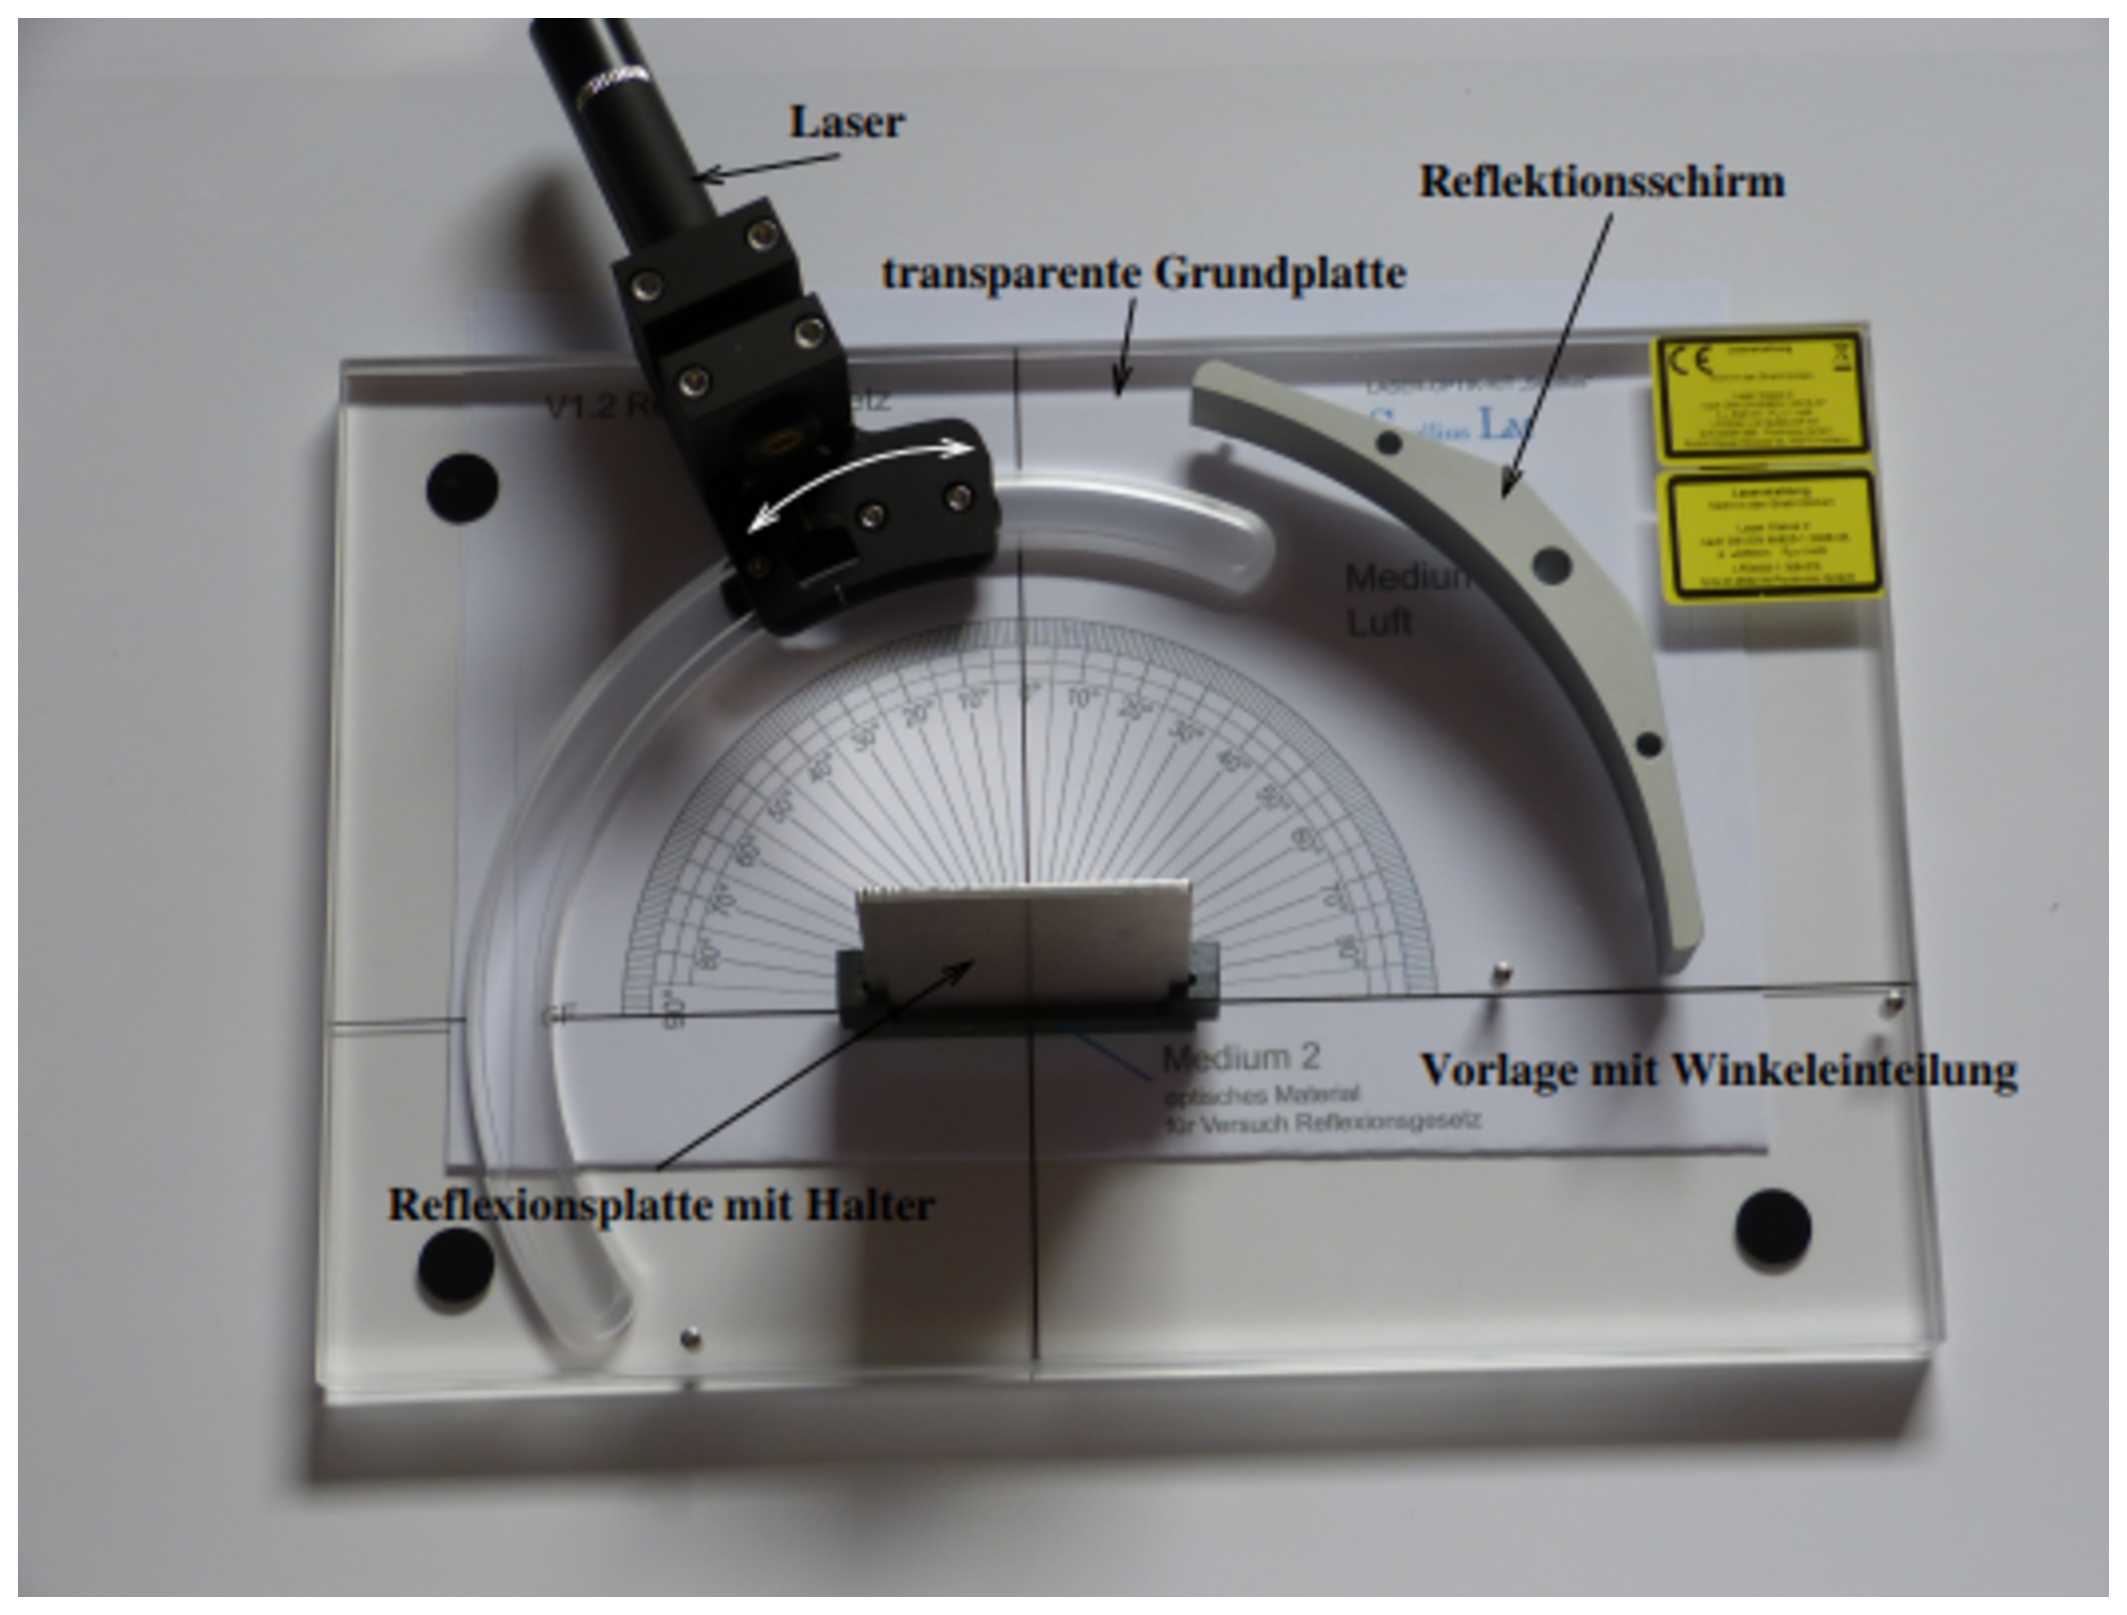
\includegraphics[height = 6cm]{Aufbau.pdf}
    \caption{Aufbau zur Messung von Reflexion, Brechung und Beugung \cite{ap400}.}
    \label{fig:aufbau}
\end{figure}

In der Mitte des Halbkreises lassen sich verschiedene geometrische Elemente platzieren,
die in \autoref{fig:figuren} abgebildet sind. Auf der Grundplatte sind Aluminiumstifte
befestigt, die eine einfachere Anbringung der Optiken realisieren.

\begin{figure}
    \centering
    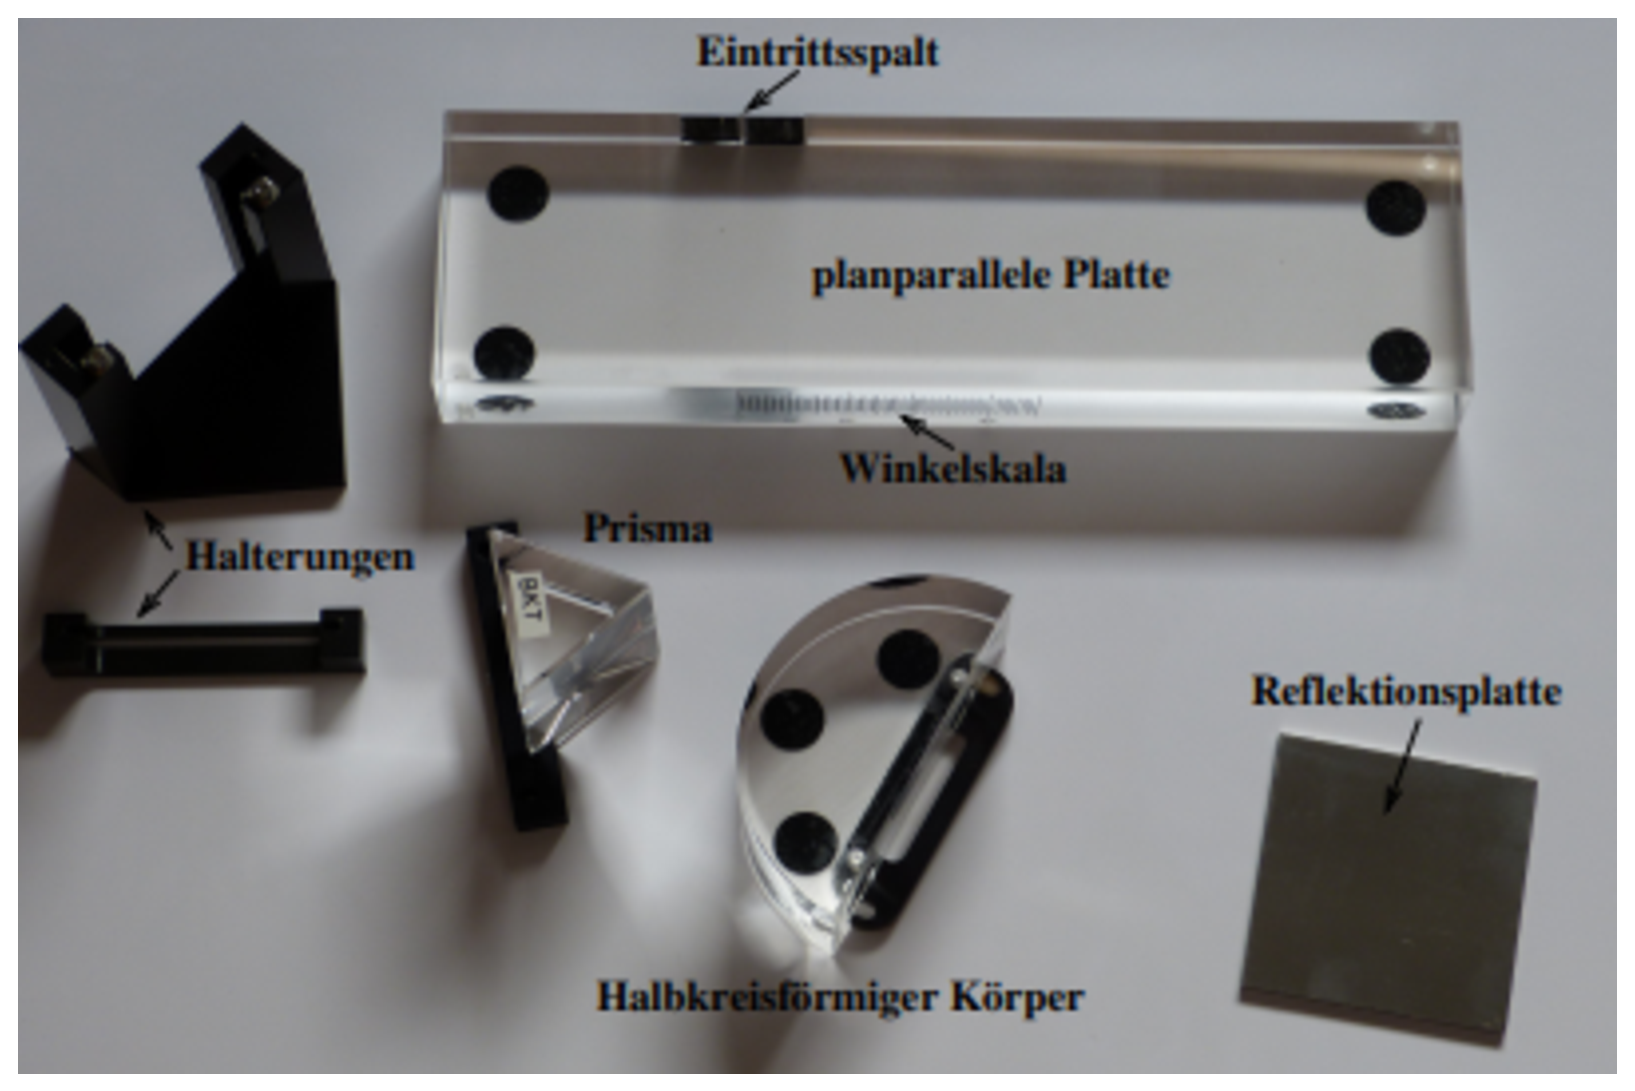
\includegraphics[height = 6cm]{Teile.pdf}
    \caption{geometrische Elemente für die Einzelversuche \cite{ap400}.}
    \label{fig:figuren}
\end{figure}

Desweiteren befindet sich an der Messapparatur ein Reflexion, der erhöht werden kann.
Bei der Untersuchung der Brechung und der Transmission kann ein Transmissionsschirm 
aufgestellt werden. Außerdem können unter die transparente Grundplatte Vorlagen für
die einzelnen Teilversuche gelegt werden.